\documentclass[hyperref=unicode]{beamer}

\usepackage[absolute,overlay]{textpos}
\usepackage{graphicx}
\usepackage{adjustbox}
\usepackage{chemfig}
\usepackage[version=4]{mhchem}
\usepackage{wrapfig}
\usepackage{multirow}
\adjustboxset*{center}
\usepackage{caption}
\usepackage{chemformula}
\usepackage{elements}

%dělení slov
\usepackage{ragged2e}
\let\raggedright=\RaggedRight
%konec dělení slov

\usepackage{fontspec}
\usepackage{unicode-math}

\usepackage{polyglossia}
\setdefaultlanguage{czech}

\def\uv#1{„#1“}

\mode<presentation>{\usetheme{Madrid}}
\DefineNamedColor{named}{pozadi}{RGB}{200,200,200}
\usecolortheme{crane}

\setbeamertemplate{footline}[frame number]

\addtobeamertemplate{frametitle}{
	\let\insertframetitle\insertsectionhead}{}
\addtobeamertemplate{frametitle}{
	\let\insertframesubtitle\insertsubsectionhead}{}

\makeatletter
\CheckCommand*\beamer@checkframetitle{\@ifnextchar\bgroup\beamer@inlineframetitle{}}
\renewcommand*\beamer@checkframetitle{\global\let\beamer@frametitle\relax\@ifnextchar\bgroup\beamer@inlineframetitle{}}
\makeatother
\setbeamercolor{section in toc}{fg=blue}
\setbeamertemplate{section in toc shaded}[default][100]

\title[Crisis] % (optional, only for long titles)
{Termodynamika}

\subtitle{Vnitřní energie, entalpie, entropie, termochemie}

\date{}

\titlegraphic{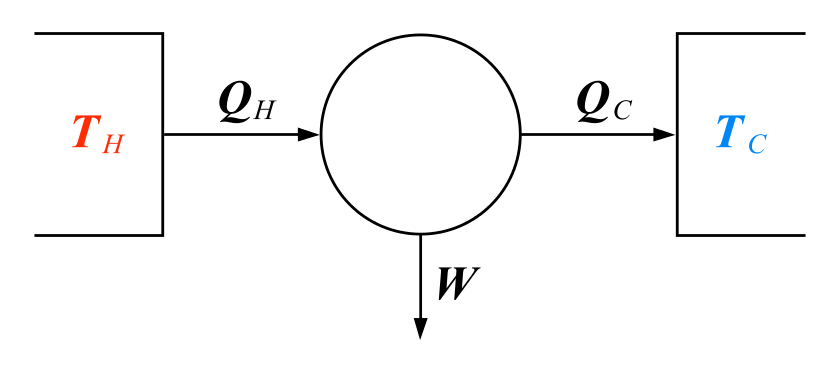
\includegraphics[keepaspectratio,width=8cm]{carnot.png}}
\begin{document}

\frame{\titlepage}

\section{Termodynamika}
\frame{
	\frametitle{}
	\vfill
Energetické přeměny při chemických a fyzikálních procesech,
přenos energie mezi látkami, vzájemné přeměny různých druhů
energie.
	\begin{itemize}
	\item Rozhoduje pouze počáteční a konečný stav.
	\item Nezávisí na mechanismu změny.
	\item Předpověď směru, samovolnosti a rozsahu reakcí.
	\item Nepočítá s časem, neurčí rychlost nebo mechanismus děje.
	\end{itemize}
	\vfill
}

\frame{
	\frametitle{}
	\vfill
	\begin{itemize}
	\item Extenzivní veličiny - závisí na příspěvcích od jednotlivých částí soustavy, jsou aditivní - hmotnost, elektrický náboj, látkové množství, ...
	\item Intenzivní veličiny - nejsou aditivní - teplota, tlak, viskozita, koncentrace, hustota, ...
	\item Stav systému - je popsán intenzivními veličinami (T, p, c).
	\item Stavová funkce - fyzikální charakteristika, jejíž hodnota závisí na stavu soustavy.
	\end{itemize}
	\vfill
}

\frame{
	\frametitle{}
	\vfill
	\begin{itemize}
	\item Izolovaný systém - nevyměňuje s okolím ani energii, ani hmotu.
	\item Uzavřený systém - vyměňuje s okolím energii.
	\item Otevřený systém - vyměňuje s okolím energii i hmotu.
	\item Teplota - pravděpodobnostní veličina, popisuje makroskopické systémy.
	\item Teplo - část vnitřní energie.
	\end{itemize}
	\vfill
}

\subsection{Termodynamické zákony}
\frame{
	\frametitle{}
	\vfill
	\begin{itemize}
	\item Nultý: Jsou-li dvě a více těles v termodynamické rovnováze s tělesem dalším, pak jsou všechna tato tělesa v rovnováze.
	\item První: Celkové množství energie (všech druhů) izolované soustavy zůstává zachováno.
	\item Druhý
	\begin{itemize}
		\item Teplo nemůže při styku dvou těles různých teplot samovolně přecházet z tělesa chladnějšího na těleso teplejší.
		\item Nelze sestrojit periodicky pracující tepelný stroj, který by trvale konal práci pouze tím, že by ochlazoval jedno těleso, a k žádné další změně v okolí by nedocházelo.
	\end{itemize}
	\item Třetí: Čistou pevnou látku nelze konečným pochodem ochladit na teplotu absolutní nuly (0 K; -273,15 \textcelsius), k této teplotě se lze pouze přiblížit.
	\end{itemize}
	\vfill
}

\subsection{Vnitřní energie}
\frame{
	\frametitle{}
	\vfill
	\begin{itemize}
	\item Stavová veličina - závisí na stavu systému, ale ne na tom, jak se systém do tohoto stavu dostal.
	\item Součet kinetické a potenciální energie systému, jde o energii všech částic, ze kterých se systém skládá.
	\item $U = \sum\limits_{i=0}^{n}\frac{1}{2}m_iv_i^2 + E_p$
	\item Její absolutní hodnotu nelze změřit ani vypočítat, pouze její změny.
	\item $\Delta U = U_2 - U_1$
	\item V termodynamice platí tzv. známková konvence: \emph{To, co snižuje vnitřní energii systému, má zápornou hodnotu a to, co ji zvyšuje, má hodnotu kladnou.}
	\end{itemize}
	\vfill
}

\subsection{Objemová práce W}
\frame{
	\frametitle{}
	\vfill
	\begin{itemize}
	\item Práce vykonaná nebo přijatá při změně objemu systému.
	\item $W = F dx = pS dx = p dV$
	\item $\mathrm{d}V = S \mathrm{d}x$; S - plocha pístu
	\item Pokud systém práci koná ($dV<0$), je  W $<$ 0; pokud ji přijímá ($dV>0$) je W $>$ 0.
	\end{itemize}
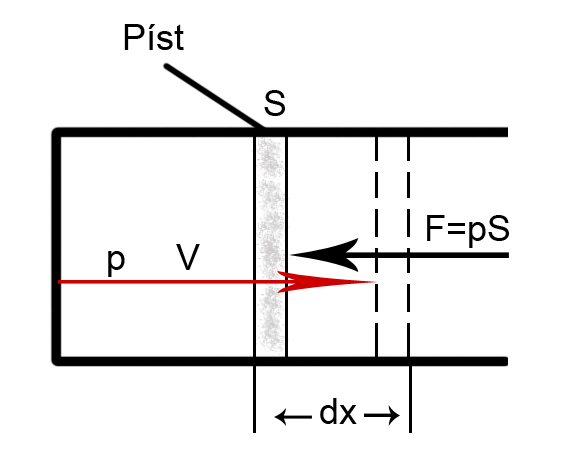
\includegraphics[keepaspectratio,width=6cm]{objemovaPrace.jpg}
	\vfill
}

\subsection{Entalpie a entropie}
\frame{
	\frametitle{}
	\vfill
	\begin{itemize}
	\item \textbf{Entalpie} (H) vyjadřuje množství energie uložené v systému.
	\item $\Delta H = \Delta U + p\Delta V$
	\item Za izobarických podmínek je entalpie rovna množství tepelné energie v systému.
	\item $\Delta H = Q$
	\item $\mathrm{d} H(S,p) = T\mathrm{d} S + V \mathrm{d} p$
	\item \textbf{Entropie} (S) popisuje neuspořádanost systému, resp. počet stavů, které může systém nabýt.
	\item $S = - k\sum\limits_i P_i \ln P_i \!$
	\item $\Delta S > 0$ - Spontánní proces
	\item $\Delta S < 0$ - Proces probíhá v opačném směru
	\item $\Delta S = 0$ - Rovnováha
	\end{itemize}
	\vfill
}

\subsection{Gibbsova energie}
\frame{
	\frametitle{}
	\vfill
	\begin{itemize}
	\item $\Delta G$ je stavová funkce
	\item $\Delta G^0$ - Gibbsova volná energie za standardních podmínek
	\begin{itemize}
		\item 298,15 K (25 \textcelsius)
		\item 100 000 Pa (1 bar) pro plyny
		\item Koncentrace roztoků 1~mol.dm$^{-3}$
	\end{itemize}
	\item Hodnoty $\Delta G^0$ jsou tabelovány
	\item \ce{C + O2 -> CO2}
	\item $\Delta G^0_{sluc} = -394,4 kJ.mol^{-1}$
	\item $\Delta G^0 = \Delta H^0 - T \Delta S^0$
	\item $\Delta G^0_{reak} = \sum \nu_{prod} \Delta G^0_{sluc}(prod) - \sum \nu_{reakt} \Delta G^0_{sluc}(reakt)$
	\item $\nu$ - stechimoterický koeficient
	\end{itemize}
	\vfill
}

\section{Termochemie}
\frame{
	\frametitle{}
	\vfill
	\begin{itemize}
	\item Reakční teplo dané reakce a reakční teplo opačné reakce jsou až na znaménka stejná.
	\item Výsledná hodnota reakčního tepla nezáleží na průběhu chemické reakce, ale pouze na jeho počátečním a konečném stavu.
	\end{itemize}
	\begin{center}
	\begin{tabular}{lr}
	Endotermní reakce & $\Delta H > 0$ \\
	Exotermní reakce & $\Delta H < 0$ \\
	Atermická reakce & $\Delta H = 0$ \\
	\end{tabular}
	\end{center}
	\begin{itemize}
	\item Pro správný výpočet reakčního tepla je nutné znát skupenství všech látek reakci.
	\item \ce{CH4(g) + 2 O2 (g) -> CO2(g) + {\color{red}\ce{2 H2O(g)}}} \hfill $\Delta H = -802\ kJ$
	\item \ce{CH4(g) + 2 O2 (g) -> CO2(g) + {\color{red}\ce{2 H2O(l)}}} \hfill $\Delta H = -890\ kJ$
	\end{itemize}
	\vfill
}

\frame{
	\frametitle{}
	\vfill
	\begin{itemize}
	\item Standardní spalné teplo - teplo, při kterém se spálí 1~mol látky v nadbytku kyslíku. Spalná tepla prvků jsou nenulová.
	\item $\Delta H^0_{298} = \sum (\Delta H^0_{sp})_{reakt} - \sum (\Delta H^0_{sp})_{prod}$
	\item Standardní slučovací teplo - teplo, při kterém vzniká 1~mol látky přímo z prvků, reakční látky musí být ve standardním stavu. Standardní slučovací tepla prvků jsou rovna nule.
	\item $\Delta H^0_{298} = \sum (\Delta H^0_{sl})_{reakt} - \sum (\Delta H^0_{sl})_{prod}$
	\end{itemize}
	\begin{center}
	\begin{tabular}{|c|c|c|}
	\hline
	\bf látka & \bf skupenství & \bf $\Delta H_f^0 [kj.mol^{-1}]$ \\
	\hline
	\ce{I2} & (s) & 0 \\
	\hline
	\ce{I2} & (g) & +62 \\
	\hline
	\ce{O2} & (g) & 0 \\
	\hline
	\ce{O3} & (g) & +142,7 \\
	\hline
	\end{tabular}
	\end{center}
	\vfill
}

\end{document}